% Generated by paper/scripts/writing_sample_exhibits.py.
\begin{figure}[t]
\centering
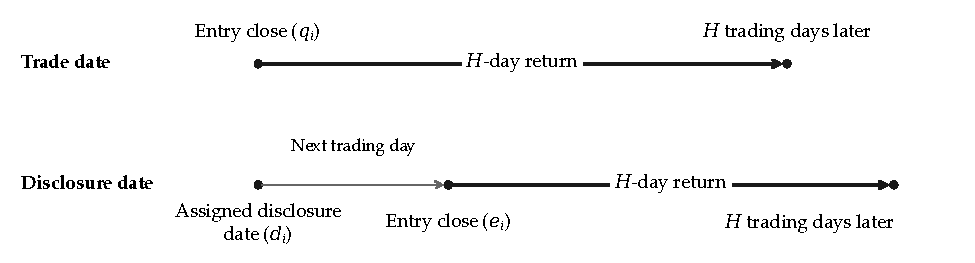
\includegraphics[width=\textwidth]{figures/writing_sample_timeline.pdf}
\caption{Trade-date and disclosure-date return windows (not to scale). The trade-date window starts at the close of $q_i$, the first trading day on or after the assigned trade date $d_i^{\mathrm{tr}}$, and the disclosure-date window starts at the close of $e_i$, the first trading day strictly after the assigned disclosure date $d_i$. Each window compounds the next $H$ close-to-close returns. The two windows measure stock performance after the reported trade and after an investor could respond to the filing, respectively.}
\label{fig:timeline}
\end{figure}
